\documentclass[dcc]{fcfmcourse}
\usepackage{teoria}
\usepackage[utf8x]{inputenc}
\usepackage{listings}
\usepackage{mathtools}

\renewcommand{\figurename}{Figura.}

\setlength{\parindent}{0pt}

\title{Tarea 4: Cálculo de derivadas usando árboles binarios}
\course[CC3001]{Algoritmos y Estructuras de Datos}
\professor{Nelson Baloian}
\professor{Patricio Poblete}
\assistant{Gabriel Azócar}
\assistant{Manuel Cáceres}
\assistant{Michel Llorens}
\assistant{Sergio Peñafiel}
% Si pasas el comando usedate a la clase, la fecha aparecerá bajo la lista de auxiliares.
% Puedes usar el formato de fecha pparéor defecto de latex (y traducirla usando babel)
% o puedes escribir lo que quieras con el comando \date.
% \date{1 de Septiembre, 2015}


\begin{document}
\maketitle
\vspace{-2ex}
\begin{center}
Fecha de Entrega: 5 de Junio  \textbf{23:30hrs} \\
\end{center}


\section{Introducción}
Como se vio en clases, un árbol binario se puede usar para guardar expresiones aritméticas. Además de la ventaja de que es fácil evaluar una expresión cuando está representada por un árbol, otra ventaja es que permite su manipulación simbólica, por ejemplo, cuando se quiere derivar la expresión almacenada. 
\newline\newline
Esta tarea se trata precisamente de construir un árbol de expresión aritmética a partir de una expresión textual (contenida en un String) escrita en notación polaca inversa, calcular su derivada respecto de una variable dada y publicar el resultado.
\newline\newline
Ejemplo de construcción de árbol: si la expresión es 2 x 3 / * y x - +, el árbol de expresión que se debe construir sería:

\begin{figure}[!h]
    \centering
    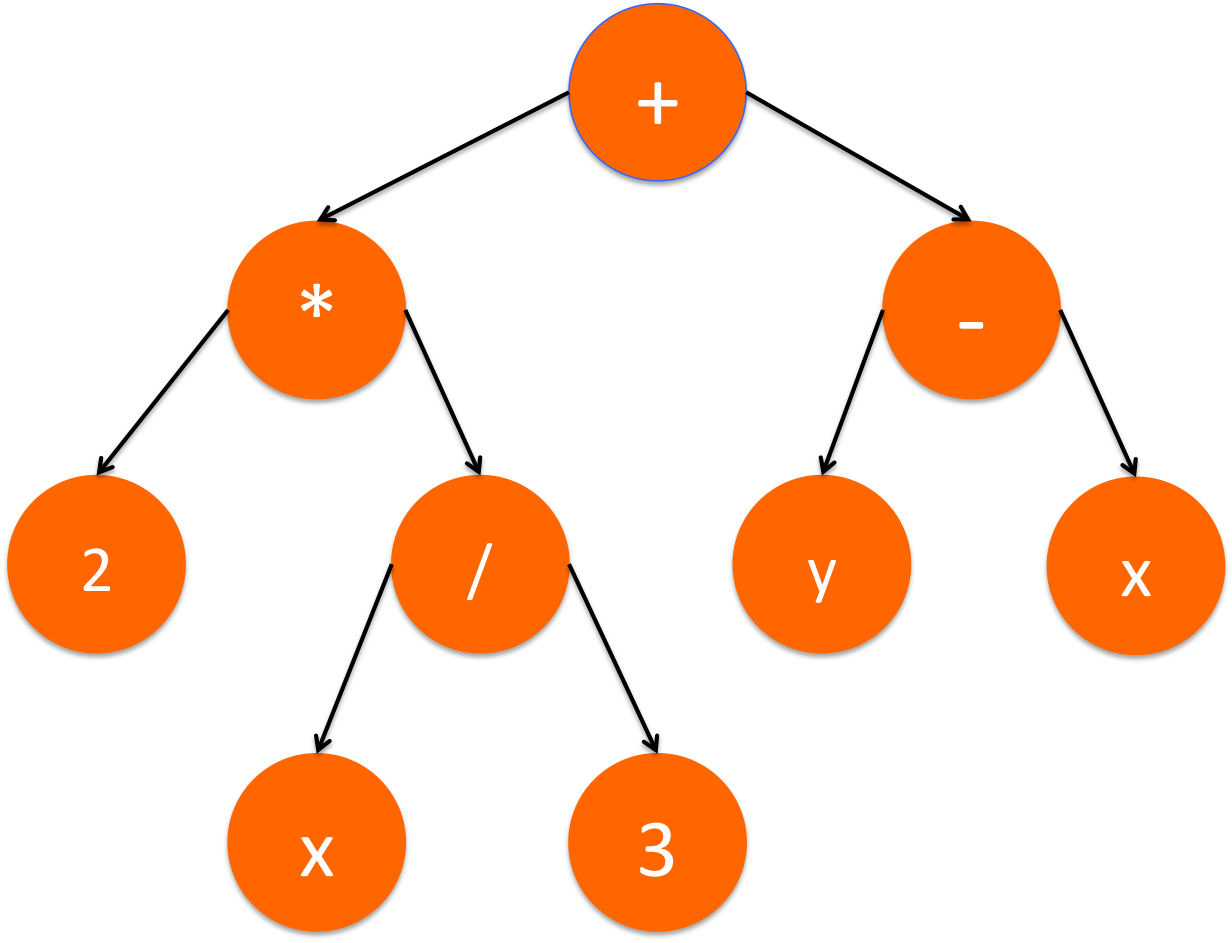
\includegraphics[scale=0.45]{imagenes/arbolDerivadas.png}
\end{figure}

\newpage
\section{Explicación}

Para obtener el árbol binario que represente la expresión, se debe construir una pila de nodo convenientemente definidos tal que al final del algoritmo la pila contenga un solo elemento que es precisamente el árbol a encontrar.
\begin{itemize}
    \item Si el símbolo que se lee es un número o una variable, se crea un nodo con ese valor y se hace push a la pila.
    
    \item Si el símbolo que se lee es una operación, entonces se crea un nodo, con el valor de esa operación, tal que sus hijos son los elementos del stack que le siguen. El siguiente elemento sería su nodo derecho y el otro el izquierdo.
    
\end{itemize}
    
Un ejemplo se visualiza en la siguiente figura, donde finalmente B es el árbol de la expresión:

\begin{figure}[!h]
    \centering
    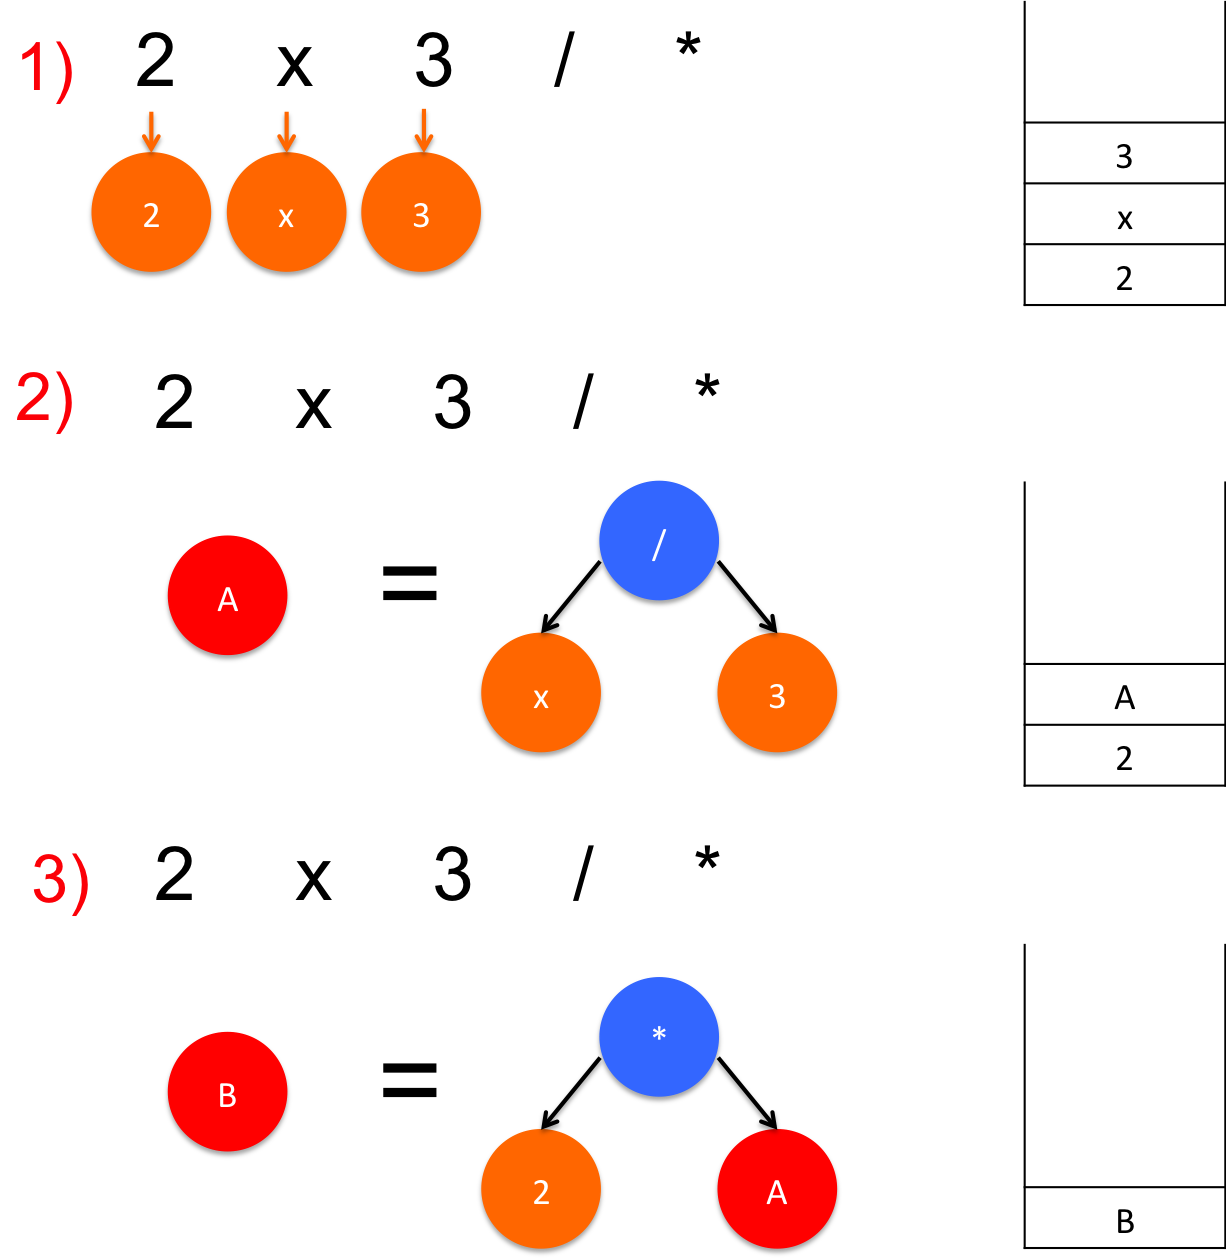
\includegraphics[scale=0.6]{imagenes/stack.png}
\end{figure}

\newpage
Para construir un nuevo árbol que contenga la expresión de la derivada de la expresión original basta aplicar las reglas de la derivación, las cuales son recursivas:
\begin{itemize}
    \item Si el nodo raíz contiene un número o una variable que no es respecto a la cual se deriva la expresión, el resultado es un nodo que contiene un cero.
    \item Si el nodo raíz contiene la variable respecto a la cual se deriva la expresión el resultado es un nodo con el número 1
    \item Si el nodo raíz contiene una operación entonces el resultado es un árbol que contiene la expresión correspondiente a la regla de la derivada para la operación: por ejemplo, para la suma es un árbol con un nodo raíz que contiene un operador de suma, el hijo izquierdo es un sub-árbol que contiene la derivada para la expresión de la izquierda y el hijo derecho es un sub-árbol que contiene la expresión de la derivada para la expresión contenida en el sub-árbol derecho. 
\end{itemize}

\section{Implementación}
Se le pide que haga un programa que lea desde el teclado primero una expresión en polaca inversa, luego el nombre de la variable con respecto  a la cual se debe derivar y responda con la expresión en in-fijo (notación aritmética normal) de dicha expresión. Esta última debe cumplir con las siguientes simplificaciones: 

\begin{itemize}
    \item Las expresiones tendrán las siguientes operaciones: suma, resta, multiplicación y división. Los símbolos serán \textbf{+}, \textbf{-}, \textbf{*} y \textbf{/} respectivamente.
    \item Las multiplicaciones de un término por 0 se deben reemplazar por 0.
    \item Las multiplicaciones de un término por 1 se deben reemplazar por el mismo término.
    \item Las sumas o restas de un término con 0 se deben reemplazar por el mismo término.
    \item Las divisiones de un término por 1 se deben reemplazar por el término.
    \item La expresión final debe omitir los paréntesis que no son necesarios. 
    \newline Por ejemplo: (((a * b) * c) + d) / e = (a * b * c + d) / e
\end{itemize}

Un ejemplo de salida simplificada sería: (2 * x) + 1 + 0 = 2 * x + 1.

Para esto, su programa debe seguir la siguiente dinámica:
\begin{enumerate}

    \item Construir el árbol de la expresión utilizando una pila, como se explicó en la sección anterior.
    
    \item Construir el árbol de la expresión derivada.
    
    \item Recorrer este último convenientemente para imprimir la expresión solicitada.
\end{enumerate}

Para simplificar el problema puede suponer lo siguiente: 
\begin{itemize}
    \item Los nombres de variables siempre tienen un solo carácter.
    
    \item Los números de la expresión serán números del 0 al 9.
    
    \item Los símbolos vienen siempre separados por un solo espacio.
    
    \item Las expresiones siempre cumplirán los supuestos de las formulas de derivación. Estas son: 
    \begin{enumerate}
        \item $({f} ± {g})' = f' ± g'$
    
        \item $({f}{g})' = f'g + fg'$
    
        \item $\left(\frac{f}{g}\right)' = \left(\frac{f'g- fg'}{g*g}\right)$
    
    \end{enumerate}
    
\end{itemize}

\section{Ejemplos de entrada y salida}

Un ejemplo de entrada y salida es el siguiente:
\newline\newline
Entrada: 2 x 3 / * y x - +
\newline\newline
Lo cual corresponde a la expresión: 2 * (x/3) + (y - x)
\newline\newline
El árbol de esta expresión es el ilustrado en la sección de Introducción.
\newline\newline
Las salidas son:
\newline
Salida derivando x: (2 * (3/3*3)) + (0 - 1) = 2 * 3/3*3 + (0 - 1)
\newline\newline
Salida derivando y: (0 + 0) + (1 - 0) = 1

\section{Condiciones de Entrega}

\begin{itemize}
    \item Esta tarea debe ser resuelta en Java.
    \item Es obligatoria la entrega de un informe en formato pdf junto con su tarea (Ver siguiente sección).
    \item Esta tarea es de carácter individual, cualquier caso de copia se evaluará con la nota mínima.
    \item No olvide subir a U-cursos todos los archivos necesarios para que su tarea funcione correctamente.
    \item Debe subir los archivos de código fuente (*.java). Los archivos compilados (*.class) no serán evaluados.
    \item Cualquier duda respecto a la tarea puede ser consultada usando el foro del curso.
    \item \textbf{NO} se aceptarán atrasos.
\end{itemize}


\section{Informe}

El informe debe describir el trabajo realizado, la solución implementada, los resultados obtenidos
y las conclusiones o interpretaciones de estos. Principalmente debe ser breve, describiendo cada uno
de los puntos que a continuación se indican:

\begin{itemize}
    \item \textbf{Portada:} Indicando número de la tarea, fecha, autor, email, código del curso, etc.
    \item \textbf{Introducción:} Descripción breve del problema y su solución.
    \item \textbf{Análisis del problema:} Exponga en detalle el problema, los supuestos que pretende ocupar, casos de borde y brevemente la metodología usada para resolverlo.
    \item \textbf{Solución del problema:} Indique claramente los pasos que siguió para llegar a la solución
    del problema. Muestre mediante figuras y ejemplos qué es lo que realiza su código. Evite
    copiar todo el código fuente en el informe, sin embargo, puede mostrar las partes relevantes
    de éste.
    \item \textbf{Modo de uso:} Explicando brevemente cualquier dato necesario para la compilación y
    ejecución de su programa.
    \item \textbf{Resultados:} Muestre ejemplos de entradas y salidas de su programa. Además muestre el resultado de los experimentos, por ejemplo, la expresión de entrada y la de salida.


\end{itemize}

\end{document}
